\documentclass[lettersize,journal,12pt]{IEEEtran}
\usepackage{fontspec}
\usepackage{amsmath,amsfonts}
\usepackage{algorithmic}
\usepackage{algorithm}
\usepackage{array}
\usepackage[caption=false,font=normalsize,labelfont=sf,textfont=sf]{subfig}
\usepackage{textcomp}
\usepackage{stfloats}
\usepackage{url}
\usepackage{verbatim}
\usepackage{xeCJK}
\usepackage{lettrine}
\usepackage{graphicx}
\usepackage{titling}
\usepackage{titlesec}
\usepackage{balance}
\usepackage{textcase}
\usepackage{setspace}
\usepackage[justification=centering]{caption}
\setmainfont{Times New Roman}[SmallCapsFont=TeX Gyre Termes:+smcp]
\newenvironment*{proof}{{\noindent\it Proof}\quad}

% rule to break words
\hyphenation{}
\def\BibTeX{{\rm B\kern-.05em{\sc i\kern-.025em b}\kern-.08em
T\kern-.1667em\lower.7ex\hbox{E}\kern-.125emX}}
\pretitle{\begin{center}\fontsize{16}{18}\selectfont\bfseries}
\posttitle{\end{center}}
\preauthor{\begin{center}\fontsize{10}{12}\selectfont}
\postauthor{\end{center}}
\predate{\begin{center}\fontsize{10}{12}\selectfont}
\postdate{\end{center}}
\titleformat{\section}
{\filcenter\fontsize{14}{16}\bfseries\uppercase}
{\thesection}
{1em}
{}
\renewenvironment{abstract}
{\fontsize{12}{14}\textit{\textbf{\abstractname---}}\bfseries\ignorespaces}
{}
\renewenvironment{IEEEkeywords}
{\fontsize{12}{14}\textit{\textbf{Keywords---}}\bfseries\ignorespaces}{}
\begin{document}
\onehalfspacing
\title{Unveiling the PageRank Algorithm: Principles, Performance, and Enhancements}
\author{Wu Zelin, Wu Zekai, Li Pengda}

\maketitle\thispagestyle{headings}
\markboth{10225101428 吴泽霖\quad10225101429 武泽恺\quad10225101460 李鹏达}{}%

\begin{abstract}
	This is the abstract area. We should write a very nb abstract here.
\end{abstract}

\begin{IEEEkeywords}
	Keyword1, Keyword2, Keyword3
\end{IEEEkeywords}


\section{Introduction}

\subsection{Background}

\lettrine{W}{ith}
the proliferation of the Internet technology, the explosively increasing amount of web pages on the World Wide Web has created the demand for the web searching engines with high-efficiency and high-effectiveness.
For the biggest search engine company Google, which held a global market share of 91.54\% until November 2023\footnote[1]{Search Engine Market Share Worldwide, Statcounter GlobalStats, 2023, https:
	//gs.statcounter.com/search-engine-market-share}, it is of primary significance to develop a powerful search algorithm to provide users with the most relevant and useful results in the shortest time.

\begin{figure}[h]
	\centering
	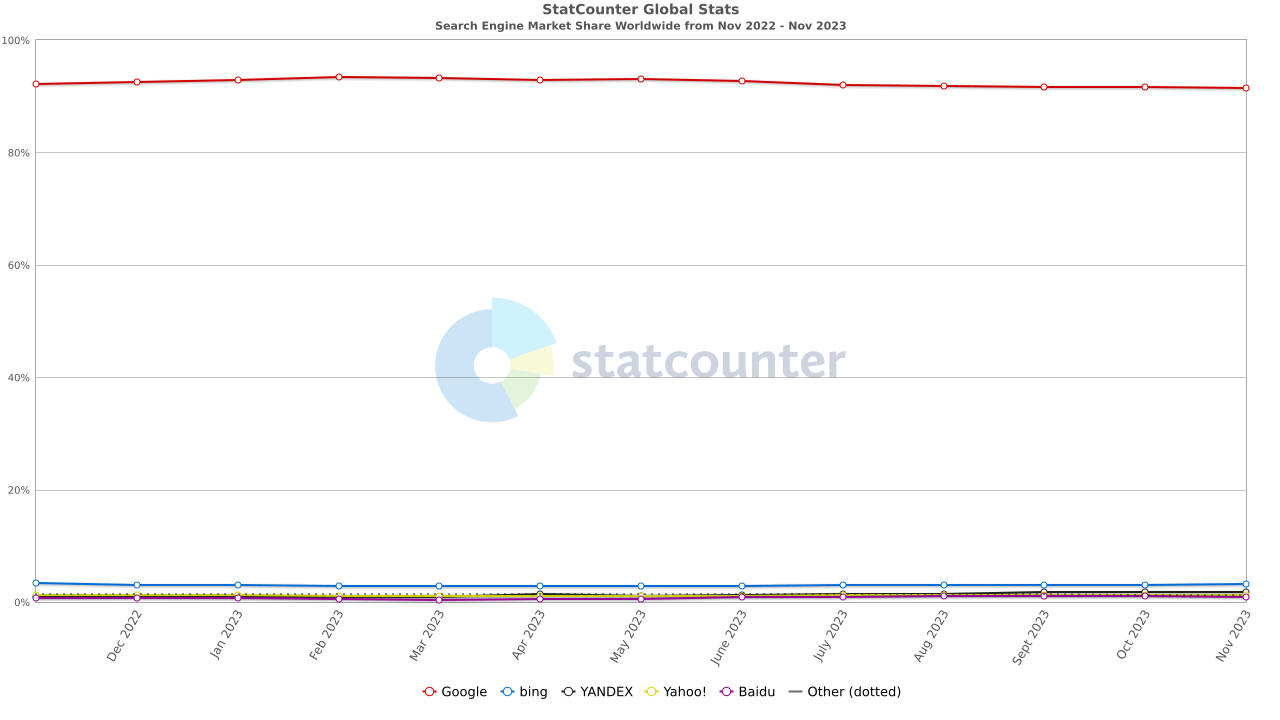
\includegraphics[width=2.5in]{images/fig2.png}
	\caption{Google's market share in the global search engine market from December 2022 to November 2023.}
	\label{fig1}
\end{figure}

Previous studies on web search algorithms have proven that TF-IDF algorithm and BM25 algorithm were efficient and effective in the early days of the Internet.

However, these algorithms have been unable to meet the growing demand of users.
The users' search queries are becoming diversified and the web pages are becoming complex.
According to the statistics, the amount of web pages, a 130-fold increase over 20 years, has surged to 130 trillion in 2016, which means it takes much longer time to search for the most relevant web pages.
To overcome the aformentioned chanllenge, Google has developed a state-of-the-art algorithm called PageRank, which is currently a fundamental algorithm in web search, redefining how we navigate web search.

\subsection{Introduction to the PageRank Algorithm}
PageRank is algorithm developed by Larry Page and Sergey Brin in the late 1990s to measure the importance of web pages.
It was originally created for the Google search engine and is named after one of the founder of Google Larry Page.
Google search engine uses the algorithm to analyze the relevance and importance of web pages and regard it as one of the factors to evaluate the effectiveness of web page optimization.

PageRank is an algorithm developed by Larry Page and Sergey Brin in the late 1990s to measure the importance of web pages.
Originally created for the Google search engine, it is named after one of the founder of Google Larry Page. Except for the searching use, the Google search engine also takes advantage of this algorithm to analyze the relevance and importance of web pages, considering it as one of the factors to evaluate the effectiveness of web page optimization.

\subsection{Outline of this Paper}

In this paper, we present the following insights and research:
\begin{itemize}
	\item The foundational principles of the PageRank algorithm.(Section 3, Subsection A)
	\item Analysis of its performance and the impact of the factors that can influence the search results and page rankings.(Section 4, Subsection A)
	\item Discussion on potential enhancements and exploration of the possibility of other factors that can improve PageRank performance.(Section 4, Subsection B)
\end{itemize}

In the next section, PageRank is briefly reviewed and analyzed.

\section{Related Work}

These section shows the brief concept of the PageRank algorithm. Theses concept motivate the design of our research.

\subsection{Synopsis of PageRank}

PageRank is a link ana1ysis algorithm and it assigns a numerical weighting to each element of hyperlinked set of documents. It is aimed to achieve the purpose of measuring the relative importance of a element of a collection. The algorithm can be applied to any collection containing mutual references between elements.We call the weight value of any element E as ``PageRank of E", which is represented symbolically as $\boldsymbol{PR(E)}$. Other factors such as ``Author Rank" can also affect the weight value of an element.

A PageRank results from a mathematical algorithm based on the webgraph, created by all World Wide Web pages as nodes and hyperlinks as edge, taking into consideration anthority hubs such as CNN. The rank value indicates an importance of a particular page. A hyperlink to this web page is called ``a vote of support for this web page". The weight of each web is defined recursively, based on the weight of all pages linking to it. For example, a page linked to many pages will have a high PageRank.

Many academic papers on PageRank existed before Page and Brin's original paper. In actual situations, PageRank is easily exploited. Relevant research tends to focus on those PageRank results affected by errors. In order to solve the problem, Google launched a new attribute nofollow for web links. The attribute allows webmasters and blogger to create some links that do not count, which means that these links do not serve as the ``vote'' so that they can ignore the spam votes.

\subsection{Markov Chain}

Markov chain, also called discrete-time Markov chain, is named after the Russian mathematician Andrei Markov. The chain is a random process in state space that undergoes a transition from a state to another. The process requires ``memoryless'' properties. That means the probability distribution of the next state can only be determined by the current state. Simultaneously, the previous events in the time series have no connection with it. The specific type of ``memoryless'' is called Markov properties. Markov chains have many applications as statistical models of real process.

At each step of the Markov chain, the system can maintain or change from one state to another according to the probability distribution. State changes are called transitions, and the probabilities associated with different state changes are called transition probabilities.

If the Markov chain runs for enough time, the distribution of its state will reach a stationary distribution and remain unchanged. Formally, if the Markov chain has $n$ states, the transition matrix is $P$
, and the stationary distribution vector is $\boldsymbol{\pi}$, then $\boldsymbol{\pi} = \boldsymbol{\pi} P$ is satisfied.

This means that the stationary distribution vector $\boldsymbol{\pi}$ is an eigenvector of the transfer matrix $P$ and corresponds to an eigenvalue of 1. Specifically, a stationary distribution has the following properties:
\begin{enumerate}
	\item [1.] $\boldsymbol{\pi_i}\geq0$, and $\sum\boldsymbol{\pi_i}=1$. That is, each element of a stationary distribution is non-negative and sums to 1, representing probability.
	\item [2.] $\boldsymbol{\pi} = \boldsymbol{\pi} P$. That is, the stationary distribution vector is the eigenvector of the transfer matrix, and the corresponding eigenvalue is 1. This shows that if the current state is stationary, then after one step of transition, the state distribution will still be stationary.
	\item [3.] Do not depend on initial state. No matter what the initial state is, after a long enough transfer, the Markov chain
	      The state distribution will reach a stationary distribution.
	\item [4.] Uniqueness. The stationary distribution of a Markov chain is unique.
\end{enumerate}

Stationary distribution represents the stable state of the Markov chain after long-term operation and will no longer be affected by the initial state.
It measures the frequency of each state in the entire chain, giving the Markov chain stable operation of each
the proportion of time spent in the state.

Assumeing that when we browse a page on the Internet, the process of selecting the next interface has no collection with that we browse before but only depends on the current page. This is a simple finite-state, discrete-time stochastic process that can be by described using a Markov chain.

\section{Main Method and Theory}



\subsection{Subsection 1}

This is a simple subsection.
We can make a citation here. \cite{ref1}

\figurename~\ref{fig2} is a figure. You can see it at the top of the page.

\begin{figure}[!t]
	\centering
	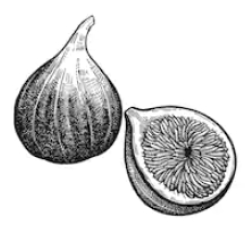
\includegraphics[width=2.5in]{images/fig1.png}
	\caption{This is a figure.}
	\label{fig2}
\end{figure}

\subsection{The 3rd Section 2nd Subsection}

This is a simple subsection too.
\section{Experiment}

This is a simple section.
\subsection{The 4th Section 1st Subsection}

This is a simple subsection.

This is an equation:

\begin{equation}
	\label{eq:1}
	e^{\pi i} + 1 = 0
\end{equation}
You can ref it by see\eqref{eq:1}.

\subsection{The 4th Section 2nd Subsection}

This is a simple subsection too.

This is a algorithm:

\begin{algorithm}[H]
	\caption{Weighted Tanimoto ELM.}\label{alg:alg1}
	\begin{algorithmic}
		\STATE
		\STATE {\textsc{TRAIN}}$(\mathbf{X} \mathbf{T})$
		\STATE \hspace{0.5cm}$ \textbf{select randomly } W \subset \mathbf{X}  $
		\STATE \hspace{0.5cm}$ N_\mathbf{t} \gets | \{ i : \mathbf{t}_i = \mathbf{t} \} | $ \textbf{ for } $ \mathbf{t}= -1,+1 $
		\STATE \hspace{0.5cm}$ B_i \gets \sqrt{ \textsc{max}(N_{-1},N_{+1}) / N_{\mathbf{t}_i} } $ \textbf{ for } $ i = 1,...,N $
		\STATE \hspace{0.5cm}$ \hat{\mathbf{H}} \gets  B \cdot (\mathbf{X}^T\textbf{W})/( \mathbb{1}\mathbf{X} + \mathbb{1}\textbf{W} - \mathbf{X}^T\textbf{W} ) $
		\STATE \hspace{0.5cm}$ \boldsymbol{\beta} \gets \left ( I/C + \hat{\mathbf{H}}^T\hat{\mathbf{H}} \right )^{-1}(\hat{\mathbf{H}}^T B\cdot \mathbf{T})  $
		\STATE \hspace{0.5cm}\textbf{return}  $\textbf{W},  \boldsymbol{\beta} $
		\STATE
		\STATE {\textsc{PREDICT}}$(\mathbf{X} )$
		\STATE \hspace{0.5cm}$ \mathbf{H} \gets  (\mathbf{X}^T\textbf{W} )/( \mathbb{1}\mathbf{X}  + \mathbb{1}\textbf{W}- \mathbf{X}^T\textbf{W}  ) $
		\STATE \hspace{0.5cm}\textbf{return}  $\textsc{sign}( \mathbf{H} \boldsymbol{\beta} )$
	\end{algorithmic}
	\label{alg1}
\end{algorithm}

\section{Experiment and results }

That's is a nibility hkafhakf

\section{Discussion on potential enhancements}

\subsection{Flaws}

Although PageRank is a classic web page ranking algorithm, it also has some flaws.

The most obvious flaw is call ``uniform access assumption''. It assumes that users have an equal probability if accessing all web pages. Apparently, it is not always true. Users' hobbies and social areas may affect this possibility.

Except the ``uniform access assumption'', there are other flaws:
\begin{itemize}
	\item Vulnerability to spam links is a serious problem. Spam links are those that exist on low-quality page or generated through SEO techniques. Their presence can influence the entire page ranking system.
	\item That the PageRank algorithm is its difficulty in handling dynamic web pages is another problem. If the content of a web page changes frequently, the PageRank algorithm may not be able to reflect these changes in a timely manner. For example, some news websites publish a large number of news every day. If the PageRank algorithm only calculates it once when the website is updated, the importance of these news will not be reflected in the ranking in time.
	\item Simultaneously, PageRank also suffers from data sparsity and lack of topics. In some cases, the PageRank may overlook some important web pages due to a lack of links to web pages relevant to the search topic. In addition, because PageRank only considers link structure and ignores the content and topic of web pages, it may not adapt well to searches in some specific areas.
\end{itemize}

\subsection{Way of Enhancements}

\subsubsection{Matrix Decomposition}
The number of web pages is extremely large on the Internet. So how to calculate the PageRank value of each page is a key issue. One way to solve the issue is to do this is to explore the specific properties of the hyperlink matrix $P$.

Consider the hyperlink matrix $P$ of the following form:

\begin{equation}
	\label{eq:114514}
	P=
	\begin{bmatrix}
		P_1    & \cdots & 0      \\
		\vdots & \ddots & \vdots \\
		0      & \cdots & P_N
	\end{bmatrix}
\end{equation}

The block $ P_I (I = 1, \ldots, N)$ on the diagonal represents the link within group $I$. We use $n_I$ to represent the number of pages within Group $I$. Each block $I$ does not communicate with the outside world, but there may be a complex relation inside.

Next, let's consider the transition matrix corresponding to the hyperlink matrix \eqref{eq:114514} $\widetilde{P} = cP  + (1-c)(1/n)E$. Let the vector $\boldsymbol{\pi}$ be the PageRank vector of the transition matrix $\widetilde{P}$, which satisfies $\boldsymbol{\pi}\widetilde{P}=\boldsymbol{\pi}, \boldsymbol{\pi e}=1$. In addition, we define the perturbation matrix of block $I$.

\begin{equation}
	\widetilde{P_I}
	=cP_I + \frac{1-c}{n_I}E
\end{equation}
Next let the vector $\boldsymbol{\pi}_I$
PageRank vector of $\widetilde{P}$, and make
\begin{equation}
	\boldsymbol{\pi}_I\widetilde{P}_I = \boldsymbol{\pi}_I, \boldsymbol{\pi}_I\boldsymbol{e}=1
\end{equation}

We can demonstrate the following formula.

\begin{equation}
	\label{eq:4444}
	\boldsymbol{\pi}=\frac{1}{n}(n_1\boldsymbol{\pi}_1,  n_2\boldsymbol{\pi}_2,\ldots,n_N\boldsymbol{\pi}_N)
\end{equation}

\begin{proof}


	denfine:
	\begin{equation}
		\widetilde{E}=
		\begin{bmatrix}
			\frac{1}{n_1}E & \cdots & 0              \\
			\vdots         & \ddots & \vdots         \\
			0              & \cdots & \frac{1}{n_N}E
		\end{bmatrix}
	\end{equation}

	To the $\boldsymbol{\pi}$ in \eqref{eq:4444}
	\begin{equation}
		\begin{aligned}
			\boldsymbol{\pi}\widetilde{P} & = \boldsymbol{\pi}[cP+(1-c)\overline{E}                                                                   \\
			                              & -(1-c)\overline{E}+(1-c)(1/n)E]                                                                           \\
			                              & =\boldsymbol{\pi}[cP+(1-c)\overline{E}]                                                                   \\
			                              & +\boldsymbol{\pi}[(1-c)\overline{E}+(1-c)(1/n)E]                                                          \\
			                              & =(\frac{n_1}{n}\boldsymbol{\pi}_1\widetilde{P_1},\ldots,\frac{n_N}{n}\boldsymbol{\pi}_N\widetilde{P_N})   \\
			                              & +(1-c)(1/n)e^T-(1-c)(1/n)e^T                                                                              \\
			                              & =\boldsymbol{\pi}=\frac{1}{n}(n_1\boldsymbol{\pi}_1,  n_2\boldsymbol{\pi}_2,\ldots,n_N\boldsymbol{\pi}_N) \\
			                              & =\boldsymbol{\pi}
		\end{aligned}
	\end{equation}

\end{proof}
Since $\widetilde{P}$ 's PageRank vector is unique, $\boldsymbol{\pi}$ is $\widetilde{P}$ 's PageRank vector.

The proof of this theorem is relatively easy. This decomposition property can also be expressed by the following formula:
\begin{equation}
	\boldsymbol{\pi}=
	\frac{1-c}{n}e^T[1-cP]^{-1}
\end{equation}

The hyperlink matrix is extremely sparse, and the time complexity is close to linear in the number of pages. Since we have broken down the hyperlink matrix, we can process each part independently and store different parts of the PageRank approximation vector in different databases to save time and space.



\subsubsection{ Topic-sensitive PageRank}

The Topic-sensitive PageRank is an extension of the PageRank algorithm.It is designed to improve the accuracy of search results. Unlike the traditional PageRank, it no longer only considers the global importance of the page, but instead ranks pages based on the importance of a given topic. This algorithm is more effective for search results that require a specific topic.
The main idea of Topic-sensitive PageRank is to build multiple PageRank vectors based on a predefined topic.Each vector has its own topic.We use them to calculate the weight of a page. In a regular keyword search query, we can use the topic of the query keyword to calculate a page's topic-sensitive PageRank score Number. In contextual search, the topic of the queried context can be used to calculate the topic-sensitive PageRank score for the page. By using these (pre-calculated) linear combinations of topic-biased PageRank vectors, it is possible to generate a context-specific page importance score at query time.This will generate more accurate ranking results than using a single generic PageRank vector.
\begin{figure*}[!t]
	\centering
	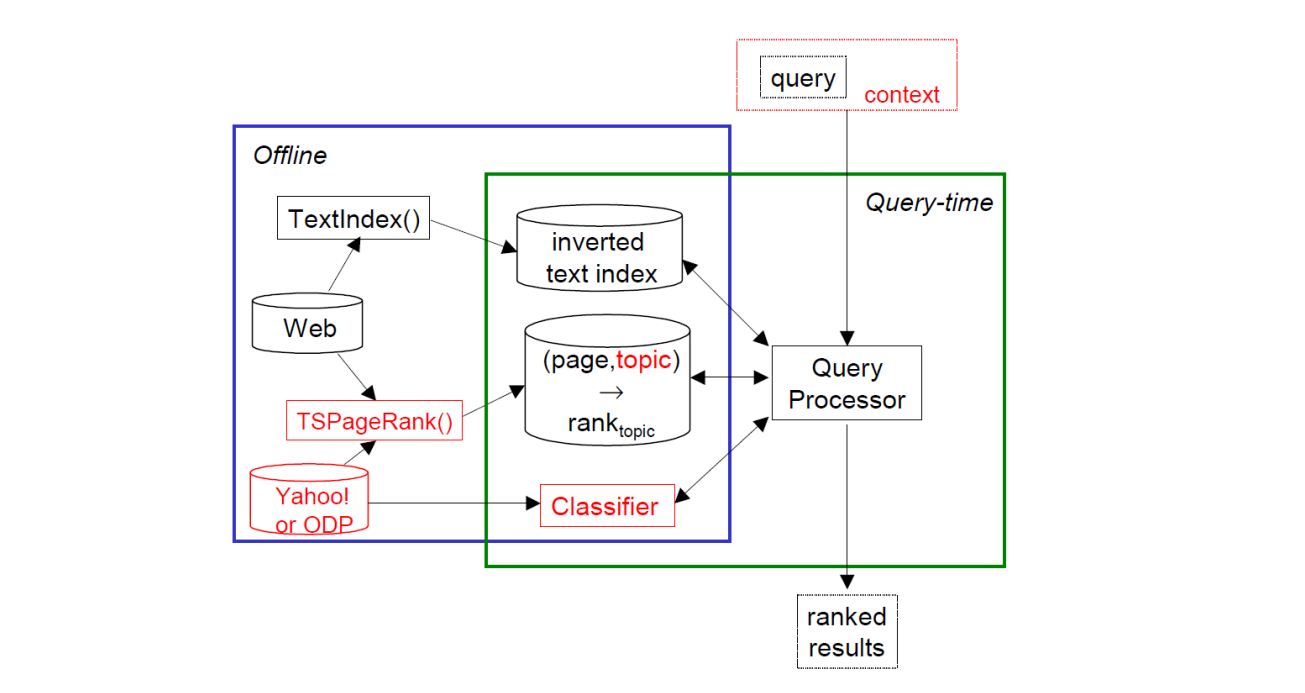
\includegraphics[width=\textwidth]{images/fig3.png}
	\caption{A system diagram that uses a subject-sensitive PageRank.}
	\label{fig3}
\end{figure*}

An overview of Topic-sensitive is provided below. During offline web crawler processing, we generated 16 topic-sensitive PageRank vectors by using top-level category URLs from OpenDirectoryProject (ODP, a web directory with more than 2.5 million URLs). At query time, we calculate the similarity of between the query (or any available context) and each topic. Then, instead of using a single global rank vector, we use topic-sensitivity linear combination of vectors, weighted using the similarity. By using a group of rank vectors, we can more accurately identify the most important pages relevant to a particular query or query context. Since link-based computation is processed offline in the preprocess, the query time cost is no higher than the normal PageRank.
\subsubsection{Sparse Matrix Optimization}
A sparse matrix or sparse array is a matrix in which most of the elements are zero in numerical analysis and scientific computing. A common criterion is that the number of non-zero elements is roughly equal to the number of rows or columns. By contrast, if most of the elements are non-zero, the matrix is considered dense.

There is an example of sparse matrix.

\begin{equation}
	A_{6\times 7}=
	\begin{bmatrix}
		0&0&1&0&0&0&0\\
		0&2&0&0&0&0&0\\
		3&0&0&0&0&0&0\\
		0&0&0&0&6&0&0\\
		0&0&0&0&0&7&4
	\end{bmatrix}
\end{equation}

The most computationally intensive part of the PageRank is to calculate the link weight between web pages that involves summing the outbound links of each web page. Since the number of outbound links for most web pages is very large, and many elements of it is zero. So, we can use the sparse matrix algorithm to solve the PageRank Matrix.That means we only need solve the zero elements.

One way to optimize a sparse matrix is to use the Compressed Sparse Row (CSR) format. In the CSR format, each non-zero element in the matrix saves its value, column index, and row offset. The row offset indicates the position of the first non-zero element in each row. The operation makes each row of the matrix can be represented by a single array. This approach can greatly reduce the computational complexity because only non-zero elements need to be processed. In the PageRank, the use of CSR format reduces computation time and memory consumption, allowing the algorithm to handle larger collections of web pages.

There is brief institution about CSR.


For a given block-size parameter $\boldsymbol{\beta}$, CSB partitions the $n\times n$
matrix $A$ into $n^2/\boldsymbol{\beta}^2$ equal-sized $\boldsymbol{\beta} \times \symbol{\beta}$ square blocks.
\begin{equation}
	\begin{pmatrix}
		A_{00}                       & A_{01}                       & \cdots & A_{0,n/\boldsymbol{\beta}-1}                      \\
		A_{10}                       & A_{11}                       & \cdots & A_{1,n/\boldsymbol{\beta}-1}                      \\
		\vdots                       & \vdots                       & \ddots & \vdots                                            \\
		A_{n/\boldsymbol{\beta}-1,0} & A_{n/\boldsymbol{\beta}-1,1} & \cdots & A_{n/\boldsymbol{\beta}-1,n/\boldsymbol{\beta}-1}
	\end{pmatrix}
\end{equation}
where the block $A_{ij}$ is the $\boldsymbol{\beta} \times \boldsymbol{\beta}$ submatrix of $A$ containing elements falling in rows $i\boldsymbol{\beta}, i\boldsymbol{\beta}+1, \ldots, (i+1)\boldsymbol{\beta}-1$ and columns
$j\boldsymbol{\beta}, j\boldsymbol{\beta}+1, \ldots, (ji+1)\boldsymbol{\beta}-1$ of the matrix. For simplicity of presentation,
we shall assume that $\boldsymbol{\beta} $is an exact power of 2 and that it divides $n$;
relaxing these assumptions is straightforward.

\section{Conclusion}

This is the conclusion area. We should write a very nb conclusion here.



\begin{thebibliography}{1}

	\bibitem{ref1}
	S. Zhan, S. Li and W. Wang, {\it{A Very Nb Book}}. Shanghai, P.R.C., East China Normal  Univ. Press, 2022.

\end{thebibliography}

\end{document}


